\documentclass{article}

% Language setting
\usepackage[english]{babel}

% Set page size and margins
\usepackage[a4paper,top=2cm,bottom=2cm,left=3cm,right=3cm,
	marginparwidth=1.75cm]{geometry}

% Useful packages
\usepackage{amsmath}
\usepackage{graphicx}
\usepackage[colorlinks=true, allcolors=blue]{hyperref}

\usepackage{footmisc}

\usepackage{tikz}
\usetikzlibrary{shapes,arrows,positioning,fit,backgrounds}

\title{
	Evaluating the Vertical and Horizontal Read and Write Scalability of 
	MobilityDB
	\\[1ex] \large Bachelor's Thesis Exposé}
\author{Eryk Karol Kściuczyk}
\date{} % This removes the date

\begin{document}
\maketitle

\vspace*{-0.3cm}

% Context
Spatio-temporal databases are increasing in popularity due to increased
production of such data by numerous IoT devices.
As the need for such databases increases, developers try to reach for 
familiar and open-source solutions.
MobilityDB, built on top of the spatial extension PostGIS, extends PostgreSQL's 
capabilities regarding spatio-temporal aspects.
Previous research has shown that the MobilityDB extension can be partially used
in conjunction with Citus, a PostgreSQL extension, which provides horizontal
scalability options.

% Problem Statement
While specific queries runtimes of BerlinMOD benchmark have been 
evaluated on 4 and 28 node clusters,
horizontal and vertical scalability of the platform has not yet been fully
explored, especially write performance.
BerlinMOD queries are not designated for distributed MOD and different set of
queries is required to further assess its performance.
Moreover, benchmarking with a wider range of cluster sizes is necessary to 
establish the scalability pattern.

% Solution Approach
In this thesis we aim to benchmark the vertical and horizontal scalability
using generated spatio-temporal data to measure metrics like request 
latency, query runtime, and read/write throughput under different data sizes.
% Aspired Implementation
We will generate data for the benchmark using a custom data generation tool
specifically developed for this study.
The tool will simulate the movement of birds, chosen due to their
seasonal migration patterns, localized movements within standard habitats,
varying flight heights and times. The benchmarking setup can be seen on figure
\ref{fig:bench_setup}.
%
We will compare the performance of MobilityDB combined with Citus on different
hardware configurations using Google Compute Engine service on Google Cloud
Platform.
Additionally, we will evaluate several scenarios, including vertically scaling 
a single node and scaling out by distributing MobilityDB across several
instances. 
Afterwards, we will compare scalability trade-offs between those two
approaches.

\begin{figure}[ht]
    \centering
    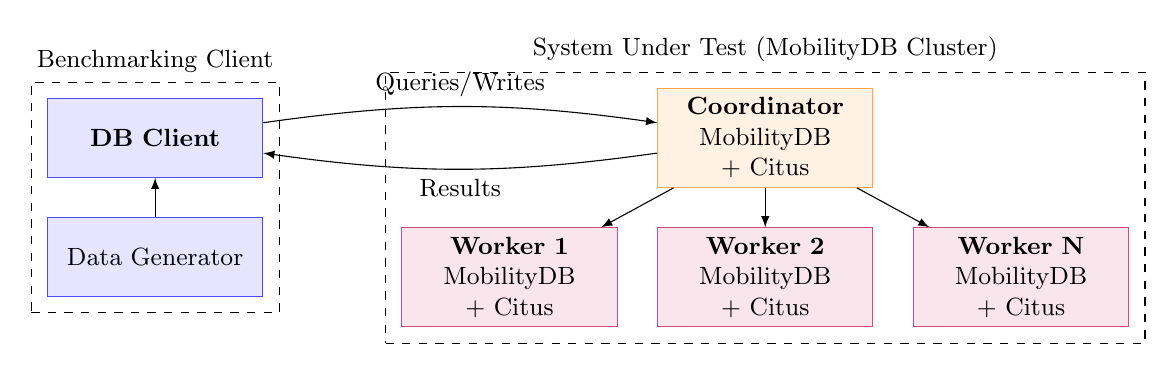
\begin{tikzpicture}[
	font=\small,
        node distance=0.5cm,
        box/.style={
            rectangle,
            draw,
            text width=2.5cm,
            minimum height=1cm,
            align=center
        },
        client/.style={
            box,
            fill=blue!10,
            draw=blue!70
        },
        coordinator/.style={
            box,
            fill=orange!10,
            draw=orange!70,
        },
        worker/.style={
            box,
            fill=purple!10,
            draw=purple!70
        },
        group/.style={
            rectangle,
            draw,
            dashed,
            inner sep=0.2cm
        },
        arrow/.style={
            ->,
            >=latex
        }
    ]
    % Client components
    \node[client] (db_client) {\textbf{DB Client}};
    \node[client, below=of db_client] (datagen) {Data Generator};
    % Client connections
    \draw[arrow] (datagen) -- (db_client);
    % Coordinator node
    \node[coordinator, right=5cm of db_client] (cn) {
         \textbf{Coordinator}\\MobilityDB \\+ Citus};
    % Worker nodes
    \node[worker, below=of cn] (w2) {
	    \textbf{Worker 2}\\MobilityDB \\+ Citus};
    \node[worker, left=of w2] (w1) {
	    \textbf{Worker 1}\\MobilityDB \\+ Citus};
    \node[worker, right=of w2] (w3) {
	    \textbf{Worker N}\\MobilityDB \\+ Citus};
    % Connections to workers
    \draw[arrow] (cn) -- (w1);
    \draw[arrow] (cn) -- (w2);
    \draw[arrow] (cn) -- (w3);
    % Client to SUT connections
    \draw[arrow] (db_client) to[bend left=8] node[above] {Queries/Writes} (cn);
    \draw[arrow] (cn) to[bend left=8] node[below] {Results} (db_client);
    
    % Group boxes
    \begin{pgfonlayer}{background}
        \node[group, fit=(db_client) (datagen)] (client) {};
        \node[above] at (client.north) {Benchmarking Client};

        \node[group, fit=(cn) (w1) (w2) (w3)] (sut) {};
        \node[above] at (sut.north) {System Under Test (MobilityDB Cluster)};
    \end{pgfonlayer}
    \end{tikzpicture}
    \caption{
	Benchmarking client will write generated bird movement data and execute
	the workload against System Under Test (MobilityDB cluster).
	The cluster consists of a coordinator and multiple workers, each running
	PostgreSQL with MobilityDB and Citus extensions. 
    }
    \label{fig:bench_setup}
\end{figure}

% Analysis/ Evaluation
% TODO:
We will measure query latencies and throughput using confidence
intervals (95\% CI) to account for performance variability in distributed
systems. 
%
To visualize the distribution of latencies across different scaling
configurations, we will utilize Empirical Cumulative Distribution Function
(ECDF) plots, to reveal performance patterns and tail latencies.
%
In order to validate the statistical significance of performance differences
between vertical and horizontal scaling approaches, we will conduct paired
t-tests where appropriate.
%
We are going to run each benchmark configuration multiple times to ensure statistical
reliability.
\end{document}
